\begin{figure}[H]
\centering
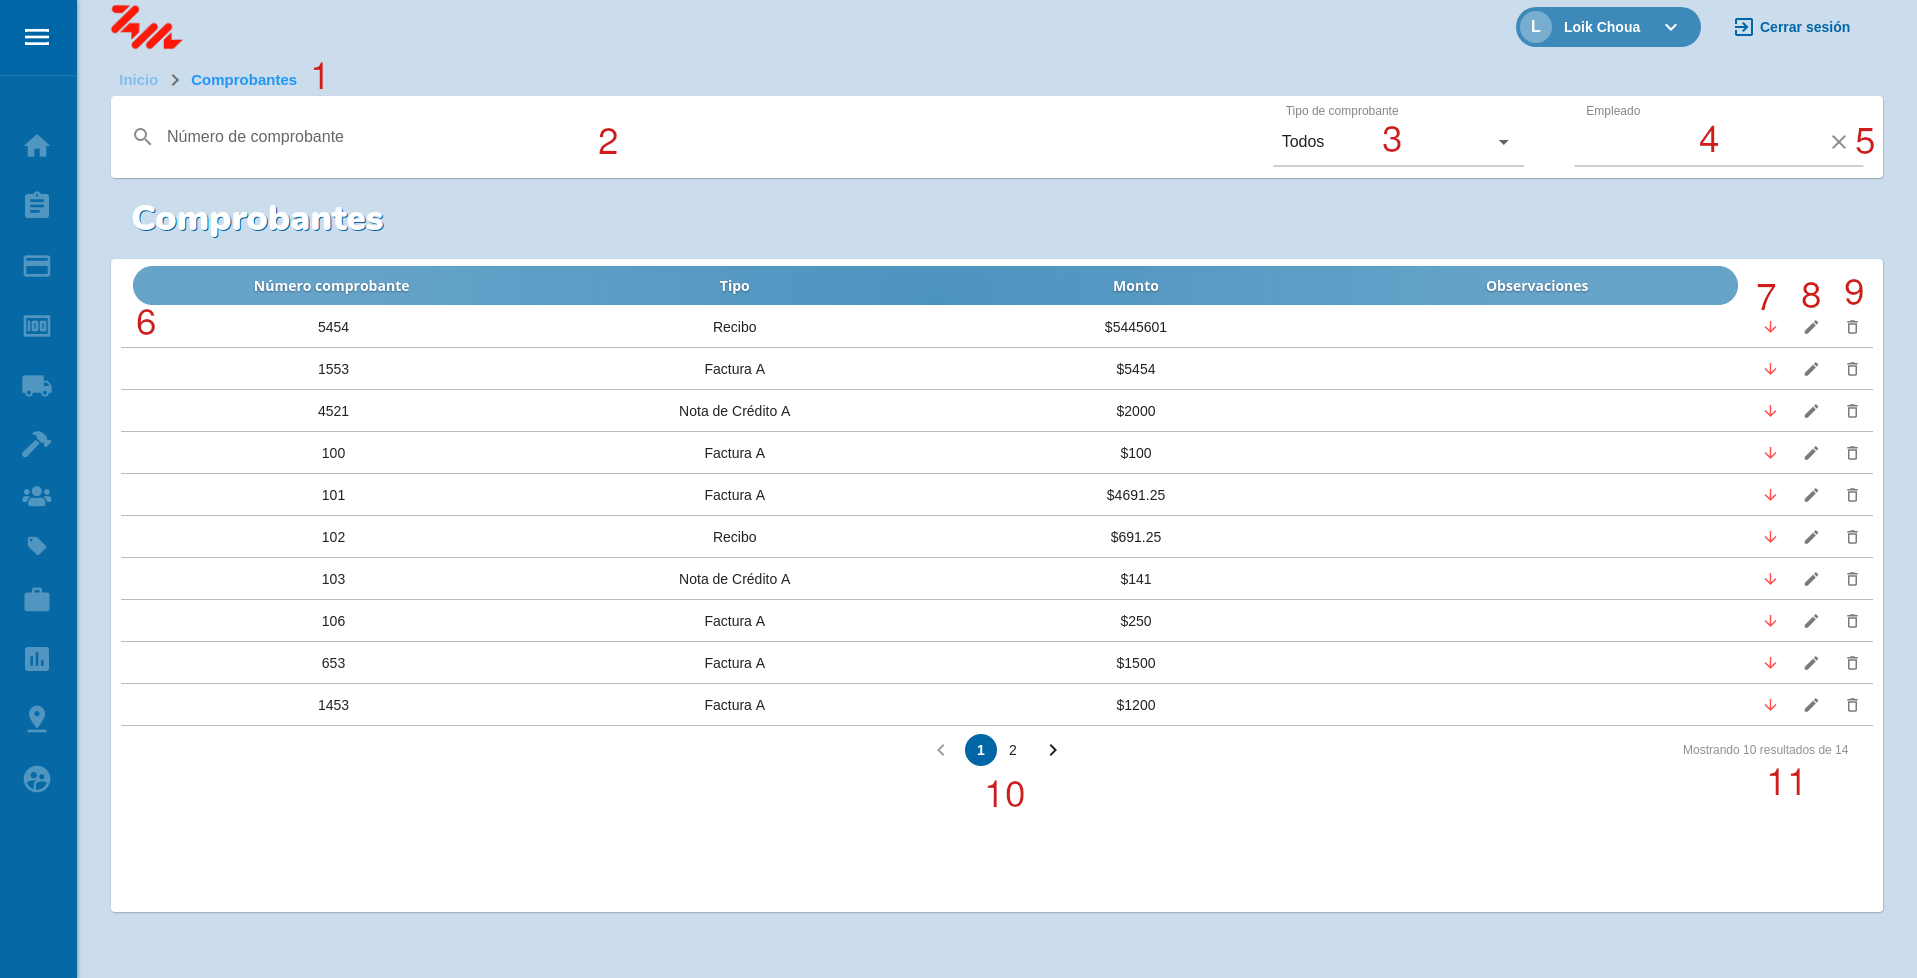
\includegraphics[width=\textwidth,height=\textheight,keepaspectratio]{Escenarios/AD-14-00}
\caption{Escenario - AD-14-00}
\label{fig:AD-14-00}
\end{figure}
Este escenario muestra toda la información referida a los comprobantes, junto con las acciones disponibles.
El botón \textbf{AD-14-01} permite navegar al escenario \textbf{AD-02-00}. El campo \textbf{AD-10-02} permite filtrar los comprobantes por su número de identificación. La lista desplegable \textbf{AD-14-03} permite filtrar a los comprobantes de acuerdo al tipo. El campo \textbf{AD-14-04} permite al usuario buscar comprobantes de acuerdo al empleado que la realizó. El campo \textbf{AD-15-04} cuenta con el boton \textbf{AD-14-05} que permite eliminar el empleado seleccionado en el campo \textbf{AD-14-05}.
El campo \textbf{AD-14-06} muestra la información relacionada a los comprobantes especificando el código de identificación, el tipo , el monto del comprobante y observaciones El botón \textbf{AD-14-07} permite al usuario dar de baja un comprobante, el botón \textbf{AD-14-08} permite al usuario editar el comprobante navegando al escenario \textbf{AD-15-00} y el botón \textbf{AD-14-09} permite al usuario borrar el comprobante. 
En  \textbf{AD-14-10} se mostrarán las páginas de resultado, pudiendo cambiar de página. En \textbf{AD-14-11} se mostrará cuantos resultados se están visualizando y el total.
\clearpage
